\documentclass[oneside,header=auto]{liverpoolthesis}
% Select the discipline once; the template chooses a suitable bibliography
% style. General or unknown disciplines fall back to APA. An explicit
% style=... option can override the automatic choice when required.
\usepackage[discipline=computer-science]{liverpoolthesis}

% Controls which heading levels are numbered. The default 4 numbers chapters,
% sections and subsections; use -1 to suppress all heading numbers.
\setcounter{secnumdepth}{4}

% ---------- Template-documentation metadata ----------
\title{University of Liverpool PhD Thesis LaTeX Template Guide}
\author{Template Documentation}
% Replace your faculty, school and degree with the correct values for your thesis.
\faculty{Faculty of Science and Engineering}
\school{School of Computer Science and Informatics}
\degree{Doctor in Philosophy}
\date{July 2026}
\subject{Instructions and examples for the University of Liverpool PhD thesis template}
\keywords{doctoral thesis, LaTeX, University of Liverpool, template guide}

\begin{document}

\frontmatter
\maketitle

\begin{abstract}
This document is both the user guide and the working example for the University of Liverpool PhD thesis LaTeX template. It demonstrates the required title-page information, preliminary pages, Roman and Arabic page numbering, chapter structure, figures, tables, mathematics, algorithms, source code, references and appendices. Candidates should replace the explanatory material with their own thesis and confirm discipline-specific conventions with their supervisor.
\end{abstract}

\begin{declaration}
% \content{
% Customized declaration content.
% }
\signature{uol-figures/signature.png}
\signdata{16 July, 2025}
\end{declaration}

\begin{acknowledgements}
Use this optional section to acknowledge supervision, funding, facilities, collaboration and personal support. Keep acknowledgements professional and check whether a funder requires a particular grant statement.
\end{acknowledgements}

\begin{publications}
  \item \publication{lamport1994}
  \item \publication{uolhistory}
\end{publications}

\tableofcontents
\listoffigures
\listoftables

\begin{abbreviations}
  \item[AI] Artificial intelligence
  \item[PGR] Postgraduate researcher
  \item[UoL] University of Liverpool
  \item[$\alpha$] Example mathematical symbol
\end{abbreviations}

\mainmatter

\chapter{About This Template}

\section{Purpose and scope}

This guide follows the organisation of established scholarly author guides: it starts with a minimal document structure, explains each supported component, and finishes with submission checks and reusable source examples. The class encodes a consistent A4 thesis layout, but it does not replace the University's current PGR guidance or advice from a School or supervisor \citep{uolformatting}.

The source of this guide is intentionally written as ordinary LaTeX. Authors can copy a demonstrated construct directly, replace its content, and remove the surrounding explanatory prose. Commands intended to be edited are kept in \texttt{example.tex}; layout decisions belong in \texttt{liverpoolthesis.cls} and \texttt{liverpoolthesis.sty}.

\section{The University of Liverpool}

The University began as University College, Liverpool in 1881 and was established as the University of Liverpool by Royal Charter in 1903. Its Victoria Building, opened in 1892, helped establish Liverpool's identity as the original ``redbrick'' university. Today the University describes itself as a founding member of the Russell Group with a research tradition that connects the institution to the city and to international partners \citep{uolhistory,uolresearch}.

\begin{figure}[htbp]
  \centering
  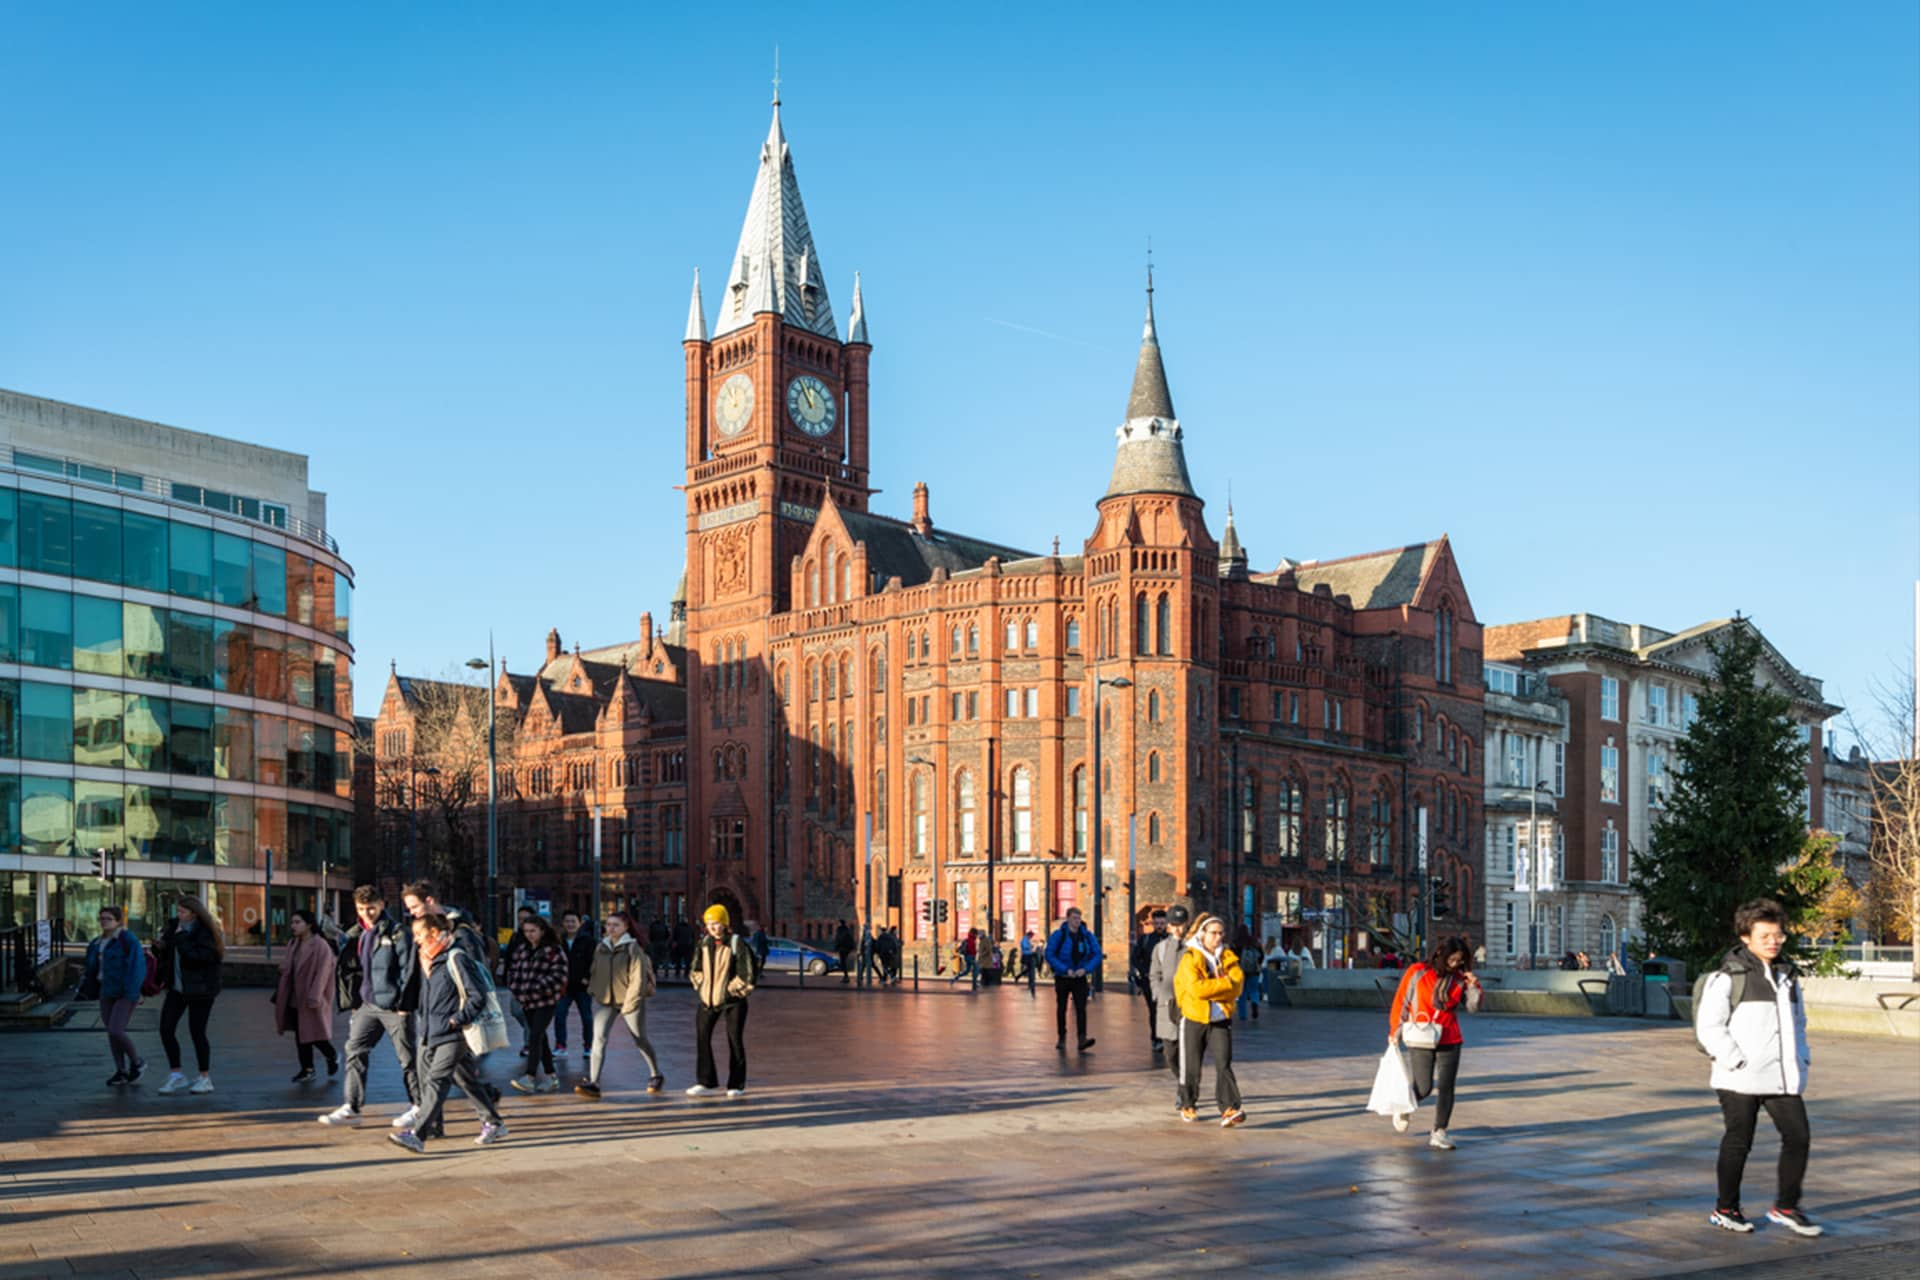
\includegraphics[width=\textwidth]{uol-figures/campus.jpg}
  \caption[University of Liverpool campus]{The University of Liverpool campus and the Victoria Building.}
  \label{fig:campus}
\end{figure}

Figure~\ref{fig:campus} also demonstrates the preferred structure of an ordinary figure: centre the graphic, place the caption below it, and add the label after the caption. Use descriptive captions that allow a reader to understand the figure without searching through the main text.

\section{Files supplied with the template}

\begin{table}[htbp]
  \centering
  \caption[Principal template files]{Principal files supplied with the template and their respective roles.}
  \label{tab:files}
  \begin{tabular}{p{0.30\textwidth}p{0.60\textwidth}}
    \toprule
    \textbf{File} & \textbf{Purpose} \\
    \midrule
    \texttt{example.tex} & Thesis content, metadata and package configuration. \\
    \texttt{liverpoolthesis.cls} & Page geometry, title page, front matter,
      numbering, fonts and PDF metadata. \\
    \texttt{liverpoolthesis.sty} & Headings, captions, tables, lists,
      theorems, algorithms, source code and discipline-aware references. \\
    \texttt{liverpoolthesis.bst} & Bundled IEEE-compatible BibTeX style used
      automatically for engineering, computing and technology disciplines. \\
    \texttt{references.bib} & Bibliographic records processed by BibTeX. \\
    \texttt{uol-figures/} & Template-owned logo and demonstration campus image. \\
    \texttt{README.md} & Concise setup, bibliography and compilation instructions. \\
    \bottomrule
  \end{tabular}
\end{table}

Keep the class, style, bibliography style and \texttt{uol-figures} directory together when moving the project. The logo is selected internally by the class and should not be specified again in the thesis source.

\chapter{Preparing the Thesis}

\section{Document declaration and metadata}

The opening block supplies the title-page text and searchable PDF information. Faculty and School names are deliberately configurable and may be left empty if they are not required.

\begin{lstlisting}[language={[LaTeX]TeX}]
\documentclass[oneside,header=right]{liverpoolthesis}
\usepackage[discipline=computer-science]{liverpoolthesis}

\title{Title of the Thesis}
\author{Full Forenames and Surname}
\faculty{Faculty Name}
\school{School, Institute or Department Name}
\degree{Doctor in Philosophy}
\date{Month Year}
\subject{Short description of the research}
\keywords{keyword one, keyword two, keyword three}

% Default: numbered chapters, sections and subsections.
\setcounter{secnumdepth}{4} % Use -1 to suppress all heading numbers.
\end{lstlisting}

For double-sided printing, replace the \texttt{oneside} and \texttt{header=right} options with \texttt{twoside} and \texttt{header=outer}; the latter places running heads at the outer edge of each printed page. The alternatives \texttt{header=left}, \texttt{header=right}, \texttt{header=inner} and \texttt{header=outer} select a fixed left position, a fixed right position, odd-left/even-right positions and odd-right/even-left positions respectively. The default \texttt{header=auto} chooses right for \texttt{oneside} and outer for \texttt{twoside}. The same selection can be made in the preamble with, for example, \verb|\thesisheaderstyle{inner}|. Chapter-opening pages retain the conventional header-free plain style.

\section{Front matter}

Place \verb|\frontmatter| before \verb|\maketitle|. The title page is counted as Roman page i but does not print the number; subsequent preliminary pages use lower-case Roman numerals. Annexe 1 requires a title page, an abstract, and a table of contents containing chapter headings, page numbers and every separate section of the thesis. The demonstration additionally includes the following useful preliminary sections where applicable:

\begin{enumerate}
  \item Abstract;
  \item Declaration;
  \item Acknowledgements;
  \item List of Publications;
  \item Table of Contents;
  \item List of Figures;
  \item List of Tables; and
  \item List of Abbreviations and Symbols.
\end{enumerate}

The abstract uses the same 12pt type and one-and-a-half line spacing as the thesis body. Annexe 1 limits it to one side of A4, normally about 450 words, and requires it to state the aims and results of the investigation \citep{uolformatting}. The declaration environment prints a doctoral-thesis declaration based on the University's current PGR Academic Integrity Policy together with the signature image and date supplied through \verb|\signature{...}| and \verb|\signdata{...}|. It distinguishes submission of thesis material for another academic award from the legitimate incorporation of published doctoral research, whose authorship and candidate contribution must be identified clearly. For campus-based PGR students the formal Academic Honesty Declaration is normally incorporated into the initial thesis submission form; candidates should confirm whether their School also expects a declaration page in the thesis \citep{uolpgrintegrity}. If an approved alternative declaration is required, uncomment \verb|\content{...}| inside the environment to replace the default text. All preliminary sections inherit the normal thesis spacing.

List publications from \texttt{references.bib} rather than retyping their details. Replace the demonstration keys with the keys for the candidate's own outputs:

\begin{lstlisting}[language={[LaTeX]TeX},caption={Generating the List of Publications from BibTeX data.}]
\begin{publications}
  \item \publication{your-first-paper}
  \item \publication{your-second-paper}
\end{publications}
\end{lstlisting}

\section{Main matter and chapter files}

Place \verb|\mainmatter| immediately before the first chapter. Arabic page numbering then restarts at 1. A long thesis is easier to maintain when chapters are stored in separate files:

\begin{lstlisting}[language={[LaTeX]TeX},caption={Including separate chapter files.}]
\mainmatter
\include{chapters/introduction}
\include{chapters/literature-review}
\include{chapters/methodology}
\include{chapters/results}
\include{chapters/conclusions}
\end{lstlisting}

Each included file should normally begin with \verb|\chapter{...}| and should not contain another \verb|\documentclass| or \verb|\begin{document}| command.

\chapter{Text, Mathematics and Lists}

\section{Headings and paragraphs}

Use numbered \verb|\chapter|, \verb|\section| and \verb|\subsection| commands to express the logical hierarchy. Avoid manual font-size and colour commands in headings: the style file applies the Liverpool blue hierarchy consistently and creates navigable PDF bookmarks.

The preamble setting \verb|\setcounter{secnumdepth}{4}| prints numbers on chapters, sections and subsections. Thus \verb|\chapter{Introduction}| begins with ``1. Introduction''. Use 3 for chapters and sections, 2 for chapters only, 1 for sections and subsections without chapter numbers, 0 for sections only, or $-1$ to suppress all heading numbers.

Start a new paragraph with a blank source line. Do not use repeated line breaks or manual vertical space to imitate paragraph spacing. The class also applies widow and orphan control, restrained emergency line breaking, and consistent spacing around displayed material.

\section{Lists}

Use the standard list environments. For example:

\begin{itemize}
  \item use \texttt{itemize} when order is not significant;
  \item use \texttt{enumerate} for a sequence or procedure; and
  \item keep items grammatically parallel and reasonably concise.
\end{itemize}

The template supplies moderate vertical separation suitable for a thesis rather than the compressed spacing common in short conference papers.

\section{Equations and cross-references}

Displayed equations should be punctuated as part of the surrounding sentence.
For example, the arithmetic mean of observations $x_1,\ldots,x_n$ is
\begin{equation}
  \bar{x}=\frac{1}{n}\sum_{i=1}^{n}x_i,
  \label{eq:mean}
\end{equation}
where $n$ is the number of observations. Refer to it with
\verb|Equation~\ref{eq:mean}|, which produces Equation~\ref{eq:mean}.

\begin{theorem}[Arithmetic--geometric mean]\label{thm:agm}
For non-negative values $x_1,\ldots,x_n$, the arithmetic mean is no smaller
than the geometric mean.
\end{theorem}
\begin{proof}
This familiar result is included only to demonstrate the theorem and proof
styles supplied by the template.
\end{proof}

Numbered theorem-style variants are available for lemmas, propositions, corollaries and conjectures. Definition-style variants cover definitions, assumptions and examples, while remarks use a lighter style. All can be referenced in the same way, for example Theorem~\ref{thm:agm}.

\chapter{Figures and Tables}

\section{Figures}

Use common PDF, PNG or JPEG graphics and size them relative to \verb|\textwidth| or \verb|\linewidth|. Preserve the image aspect ratio and ensure labels remain legible at the final printed size. Every figure must be mentioned in the text, numbered, captioned and supplied with alternative explanation in the surrounding prose where accessibility requires it. Write \verb|\caption[Short title]{Full descriptive caption}| when a concise entry is needed in the List of Figures; the optional text appears in the list, while the full caption remains with the figure.

\begin{lstlisting}[language={[LaTeX]TeX},caption={Standard figure syntax.}]
\begin{figure}[htbp]
  \centering
  \includegraphics[width=0.85\textwidth]{figures/result.pdf}
  \caption[Short result title]{A self-contained description of the result.}
  \label{fig:result}
\end{figure}
\end{lstlisting}

\section{Tables}

Use ordinary \texttt{table} and \texttt{tabular} environments. Captions appear above tables automatically. Use \verb|\caption[Short title]{Full descriptive caption}| to place the short title in the List of Tables and the full caption above the table. A caption that fits on one line is centred automatically; a caption that wraps onto multiple lines is left-aligned. The \texttt{booktabs} rules produce a clear journal-style table without vertical lines, as demonstrated in Table~\ref{tab:comparison}.

\begin{table}[htbp]
  \centering
  \caption[Comparison of methods]{Comparison of baseline and proposed methods using ordinary table syntax, with accuracy, execution time and a concise interpretation reported for each method.}
  \label{tab:comparison}
  \begin{tabular}{lrrl}
    \toprule
    \textbf{Method} & \textbf{Accuracy (\%)} & \textbf{Time (s)} &
      \textbf{Comment} \\
    \midrule
    Baseline method & 84.2 & 12.6 & Reference result \\
    Proposed method & 91.7 & 8.4 & Best overall \\
    \bottomrule
  \end{tabular}
\end{table}

For wide textual content, use fixed-width \texttt{p\{width\}} columns or the available \texttt{tabularx} environment. The optional \texttt{S} column from \texttt{siunitx} aligns decimal numbers, but it is unnecessary for simple tables.

\section{Float placement}

The placement option \texttt{[htbp]} asks LaTeX to try the current position, the top or bottom of a page, and finally a dedicated float page. Avoid forcing every float with \texttt{[H]}; allowing controlled movement usually produces better page balance. The style file permits several floats while preventing almost empty text pages and sparsely occupied float pages.

\chapter{Algorithms and Source Code}

\section{Algorithms}

Use the \texttt{algorithm} float with \texttt{algpseudocode} for procedures. Algorithms are numbered by chapter and can be referenced with ordinary \verb|\ref| commands.

\begin{algorithm}[htbp]
  \caption{Example iterative procedure}\label{alg:example}
  \begin{algorithmic}[1]
    \Require Initial value $x_0$ and tolerance $\varepsilon$
    \State $k \gets 0$
    \While{the stopping criterion is not satisfied}
      \State compute the next value $x_{k+1}$
      \State $k \gets k+1$
    \EndWhile
    \State \Return $x_k$
  \end{algorithmic}
\end{algorithm}

\section{Source code}

The \texttt{listings} configuration provides line numbers, restrained colour, automatic wrapping and an embedded monospaced font. Short fragments should support the research narrative; move extensive implementation details to an appendix or a maintained repository.

\begin{lstlisting}[language=Python,caption={Example source-code presentation.},label={lst:mean}]
def mean(values):
    """Return the arithmetic mean."""
    if not values:
        raise ValueError("values must not be empty")
    return sum(values) / len(values)
\end{lstlisting}

Algorithm~\ref{alg:example} and Listing~\ref{lst:mean} demonstrate conventional cross-references using \verb|\ref|.

\chapter{Citations, References and Appendices}

\section{Choosing a reference style}

The University requires references to be complete, consistent and presented in a form accepted within the relevant discipline; it does not impose one University-wide citation style \citep{uolformatting}. Select the discipline once and the template selects a suitable BibTeX \texttt{.bst} style:

\begin{lstlisting}[language={[LaTeX]TeX}]
\usepackage[discipline=computer-science]{liverpoolthesis}
\end{lstlisting}

The value after \texttt{discipline=} must be copied from the middle column of Table~\ref{tab:discipline-bibliography-styles}. Values are lower-case and use hyphens instead of spaces; for example, Computer Science is written exactly as \texttt{computer-science}, not \texttt{computerscience}.

\begingroup
\small
\hbadness=10000
\setlength{\LTleft}{0pt}
\setlength{\LTright}{0pt}
\captionsetup{hypcap=false}
\captionof{table}{Accepted \texttt{discipline=} values and their default
  bibliography styles.}
\label{tab:discipline-bibliography-styles}
\edef\disciplinetablenumber{\thetable}
\begin{longtable}{@{}>{\raggedright\arraybackslash}p{0.19\textwidth}
                       >{\raggedright\arraybackslash\ttfamily}p{0.58\textwidth}
                       >{\raggedright\arraybackslash}p{0.17\textwidth}@{}}
  \toprule
  \textbf{Discipline group} & \normalfont\textbf{Accepted parameter values} &
    \normalfont\textbf{Selected style} \\
  \midrule
  \endfirsthead
  \multicolumn{3}{@{}c@{}}{\normalfont Table~\disciplinetablenumber: Accepted
    \texttt{discipline=} values (continued).}\\[0.5ex]
  \toprule
  \textbf{Discipline group} & \normalfont\textbf{Accepted parameter values} &
    \normalfont\textbf{Selected style} \\
  \midrule
  \endhead
  \midrule
  \multicolumn{3}{r@{}}{\small Continued on the next page}\\
  \endfoot
  \bottomrule
  \endlastfoot
  Engineering, computing and technology &
    engineering, electrical-engineering, electronic-engineering,
    mechanical-engineering, civil-engineering, aerospace-engineering,
    chemical-engineering, materials-engineering, biomedical-engineering,
    systems-engineering, energy-engineering, computer-science, computing,
    data-science, artificial-intelligence, robotics, telecommunications &
    \normalfont IEEE numeric \\
  Medicine, health and natural sciences &
    physics, astronomy, chemistry, mathematics, statistics, medicine,
    dentistry, veterinary-science, nursing, pharmacy, public-health,
    health-sciences, life-sciences, biology, biochemistry, genetics,
    neuroscience, environmental-science, earth-sciences, geology,
    ocean-sciences, agriculture, food-science &
    \normalfont compact numeric \\
  Psychology, education, management and social sciences &
    general, psychology, education, social-sciences, sociology, anthropology,
    criminology, politics, international-relations, public-policy,
    social-work, management, business, marketing, geography, sport-science &
    \normalfont APA \\
  Economics, humanities and arts &
    economics, finance, accounting, humanities, history, archaeology,
    classics, philosophy, literature, languages, linguistics, music, arts,
    architecture, planning, communication, media-studies, theology &
    \normalfont author--year \\
  Law & law & \normalfont author--title \\
\end{longtable}
% longtable also advances the counter even though the numbered caption was
% placed above it; restore the counter for any later tables.
\addtocounter{table}{-1}
\endgroup

APA remains the fallback for \texttt{discipline=general} or an unrecognised value. A School-mandated style can override the mapping explicitly:

\begin{lstlisting}[language={[LaTeX]TeX}]
\usepackage[
  discipline=computer-science,
  style=apa
]{liverpoolthesis}
\end{lstlisting}

The selector maps the discipline to the bundled \texttt{liverpoolthesis.bst} or to a standard BibTeX style supplied by the TeX installation. The selected style is written to the auxiliary file automatically, while the references themselves remain in an ordinary \texttt{.bib} database.

Store bibliographic data in \texttt{references.bib}. Use \verb|\citep{key}| for a parenthetical citation and \verb|\citet{key}| for a textual citation; the resulting entries are formatted consistently rather than typed manually \citep{lamport1994}. Numeric bibliographies use ACM-style author/year/title sorting rather than assigning bibliography numbers by first appearance, and groups of numeric citations are automatically sorted and compressed.

\section{Printing the reference list}

The following command creates an unnumbered References chapter. The template automatically starts it on a fresh page, creates the PDF hyperlink target and adds it to the table of contents:

\begin{lstlisting}[language={[LaTeX]TeX}]
\bibliography{references}
\end{lstlisting}

\section{Appendices after references}

Appendices may follow the reference list. Use \verb|\appendix| directly and continue with ordinary chapter commands. Do not place \verb|\backmatter| before the appendices, because doing so suppresses the Appendix A, Appendix B chapter numbering provided by the base class.

\section{Theses incorporating publications}

A List of Publications does not by itself make the document a thesis that incorporates publications. Candidates using published work in place of standard chapters should agree the approach with their supervisors and follow Annexe 2 \citep{uolpublications}. In particular:

\begin{enumerate}
  \item the thesis must contain a conventional Introduction explaining the
        background and rationale;
  \item additional literature or methods chapters should supply depth and
        coherence not provided by the publications;
  \item every incorporated publication must be presented as a chapter with an
        introductory section linking it to the preceding and following work;
  \item a Conclusion must integrate the strands of all chapters and papers;
  \item each publication requires a declaration of the candidate's contribution,
        and jointly authored work requires the necessary co-author permissions;
  \item published material must be reformatted into the thesis style with
        continuous pagination, rather than inserted in the publisher's layout.
\end{enumerate}

\chapter{Pre-submission Checklist}

Before producing the examination copy, check the following items:

\begin{enumerate}
  \item Replace every placeholder in the title page and preliminary pages.
  \item Confirm the current University and School requirements.
  \item Check that the abstract fits the permitted length and page limit.
  \item Check the applicable maximum word count: Appendix 7 states that it
        includes footnotes and appendices but excludes the bibliography.
  \item Ensure every figure and table is cited, legible and correctly captioned.
  \item Resolve all missing citations, references and compilation warnings.
  \item Use one accepted reference style consistently throughout the thesis.
  \item Confirm that permissions and source acknowledgements are complete.
  \item Submit supporting material in the same PDF where practicable and consult
        the relevant Director of PGR about material that cannot be embedded.
  \item Inspect the final PDF page by page, including bookmarks, pagination,
        equations, appendices and embedded fonts.
\end{enumerate}

Automated formatting improves consistency but does not validate scholarly content. The candidate remains responsible for accuracy, attribution, accessibility and compliance with the requirements applying at submission.

\bibliography{references}

\appendix

\chapter{Minimal Thesis Skeleton}

The following skeleton shows the intended order without the explanatory content used elsewhere in this guide.

\begin{lstlisting}[language={[LaTeX]TeX},caption={Minimal document skeleton.}]
\documentclass[oneside,header=right]{liverpoolthesis}
\usepackage[discipline=computer-science]{liverpoolthesis}

\begin{document}
\frontmatter
\maketitle

\begin{abstract}
Abstract text.
\end{abstract}

\begin{declaration}
% \content{Customized declaration content.}
\signature{uol-figures/signature.png}
\signdata{16 July, 2025}
\end{declaration}

\begin{acknowledgements}
Acknowledgements text.
\end{acknowledgements}

\begin{publications}
  \item \publication{your-publication-key}
\end{publications}

\tableofcontents
\listoffigures
\listoftables

\begin{abbreviations}
  \item[UoL] University of Liverpool
\end{abbreviations}

\mainmatter
\chapter{Introduction}
Thesis text.

\bibliography{references}

\appendix
\chapter{Supplementary Material}
Appendix text.
\end{document}
\end{lstlisting}

\section{Common customisations}

Prefer semantic changes in \texttt{example.tex} and reserve visual changes for the class or companion style. This separation keeps the thesis source readable and makes global revisions predictable. If a School requires a different bibliography style, margin, heading treatment or declaration, document the reason for the change and apply it consistently rather than formatting individual pages by hand.

\end{document}
